\section{Moduler i en BMS}
For at kunne forklare de forskellige topologier er der nogle områder i en BMS der skal være styr på først. BMS'ens opgaver klares af flere moduler som ikke nødvendigvis behøver at hænge sammen. Afhængigt af den ønskede opsætning kan der være forskellige antal af de forskellige moduler. Disse moduler deles typisk ud på flere PCB'er hvis krævet, og er ofte delt op i tre forskellige: 

\subsubsection{Celleovervågningsmodul (CMU for engelsk "Cell monitoring unit")}
Dette modul er direkte forbundet til hver enkel celle. Her overvåges spænding, temperatur og andre vitale dele af cellens parametre, samt at der er her balanceringen finder sted. 

\subsubsection{Modulstyring (MMU for engelsk "Module manangement unit")}
MMU'en styrer en gruppe af de førnævnte CMU'er, og dette modul gør det derfor muligt at balancere cellerne i forhold til hinanden. 

\subsubsection{Batteripakkestyring (PMU for engelsk "Pack management unit")}
Batteripakkestyringen er det overordnede modul. Her styres MMU'erne, men samtidig holdes der også styr på hele pakkens spænding og strøm. Det er også her at sikkerhedsforanstaltningerne sidder, såsom kortslutningsbeskyttelse samt over- og afladningsbeskyttelse. Kommunikation med andre eksterne systemer foregår også her. 

\section{Centraliseret system}
I et centraliseret system er alle tre slags moduler kombineret til én enhed. De

\begin{figure}[h]
	\centering
	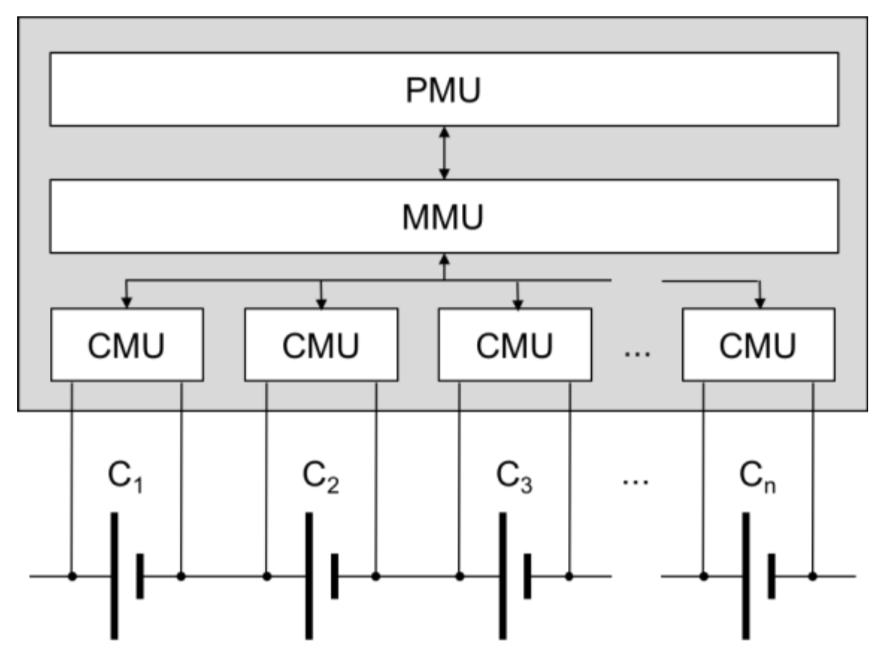
\includegraphics[width=6cm]{billeder/centralized.png}
	\caption{En centraliseret BMS}
	\label{fig:centralized_BMS}
\end{figure}

\section{Distribueret system}
I et distribueret system foretages alle målinger på den enkelte celle og kommunikerer sin status til en master enhed. Hver celle er udstyret med sin egen dedikerede CMU, MMU og PMU. De enkelte PMU'er kan kommunikere med hinanden alt afhængig af behov.
\\

Fordelen ved denne topologi er at designet er simpel og pålidelig. Ulempen er dog, at den kræver et højt antal slave enheder, som kan give problemer rent monteringsmæssigt.



\section{Modulær system}

\section{Valg af topologi}
En sammenligning mellem de 3 systemer efterfulgt af en vægtning i forhold til vores krav - 4 celler fx
\subsection{Vægtningsskema}

\begin{itemize}
	\item Virkningsgrad
	\item Sikkerhed
	\item Modularitet
	\item Brugertilpasning
\end{itemize}